\chapter{Aufbau}
\label{ch:Funktionsweise und Aufbau}
Die Funktionsweise des Gestikulasers besteht aus der Detektion und Weiterverarbeitung von Lichtsignalen, welche mit einer Geste erzeugt werden. Dabei wird infrarotes Licht von einer LED Quelle durch die Hand reflektiert und durch verschiedene Photodioden detektiert. Die durch die Photodioden erhaltenen Daten werden dann in einer Software weiterverarbeitet, welche mit Hilfe von Machine Learning die tatsächliche Handgeste erkennt. Von dort aus kann dann jedes beliebige Endgerät angesteuert werden.

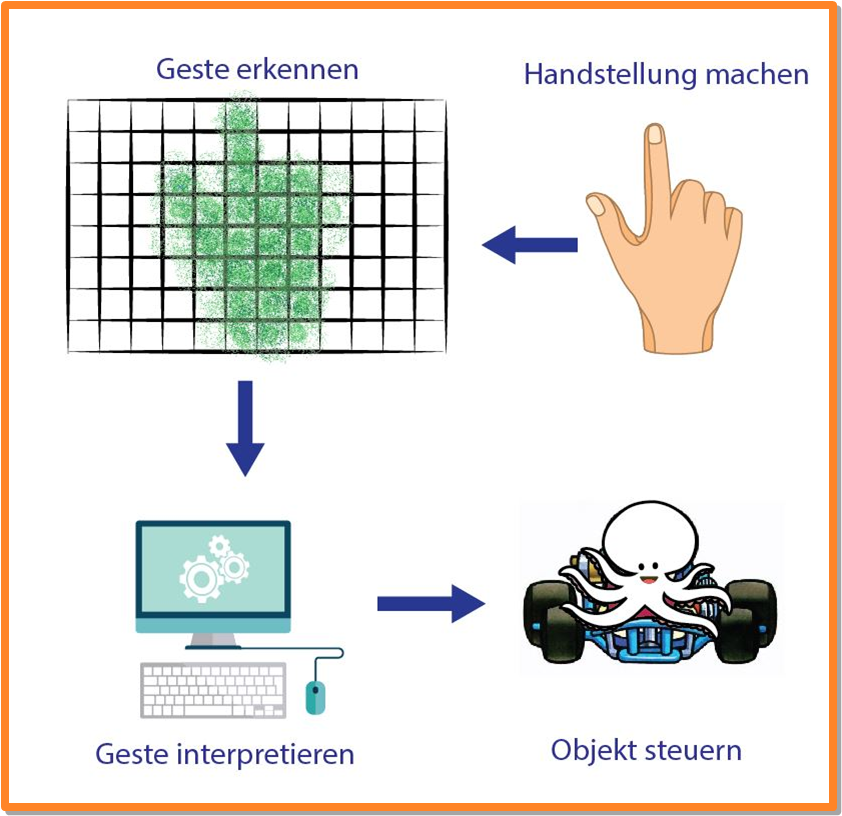
\includegraphics[scale=0.8]{figures/AblaufGestikulaser.png}

Der Gestikulaser selbst besteht aus einer Platte, der Photoplatte, welche aus verschiedenen Steckmodulen zusammen gesteckt werden kann. Die Steckmodule bestehen aus einzelnen kleinen Boxen, in welche die Elektronik integriert ist. In der Mitte befindet sich der Oktokommander, welcher durch weitere Detektormodule erweitert werden kann. Auf jedes der Module befinden sich vier Photodioden um das reflektierte Licht zu messen. 

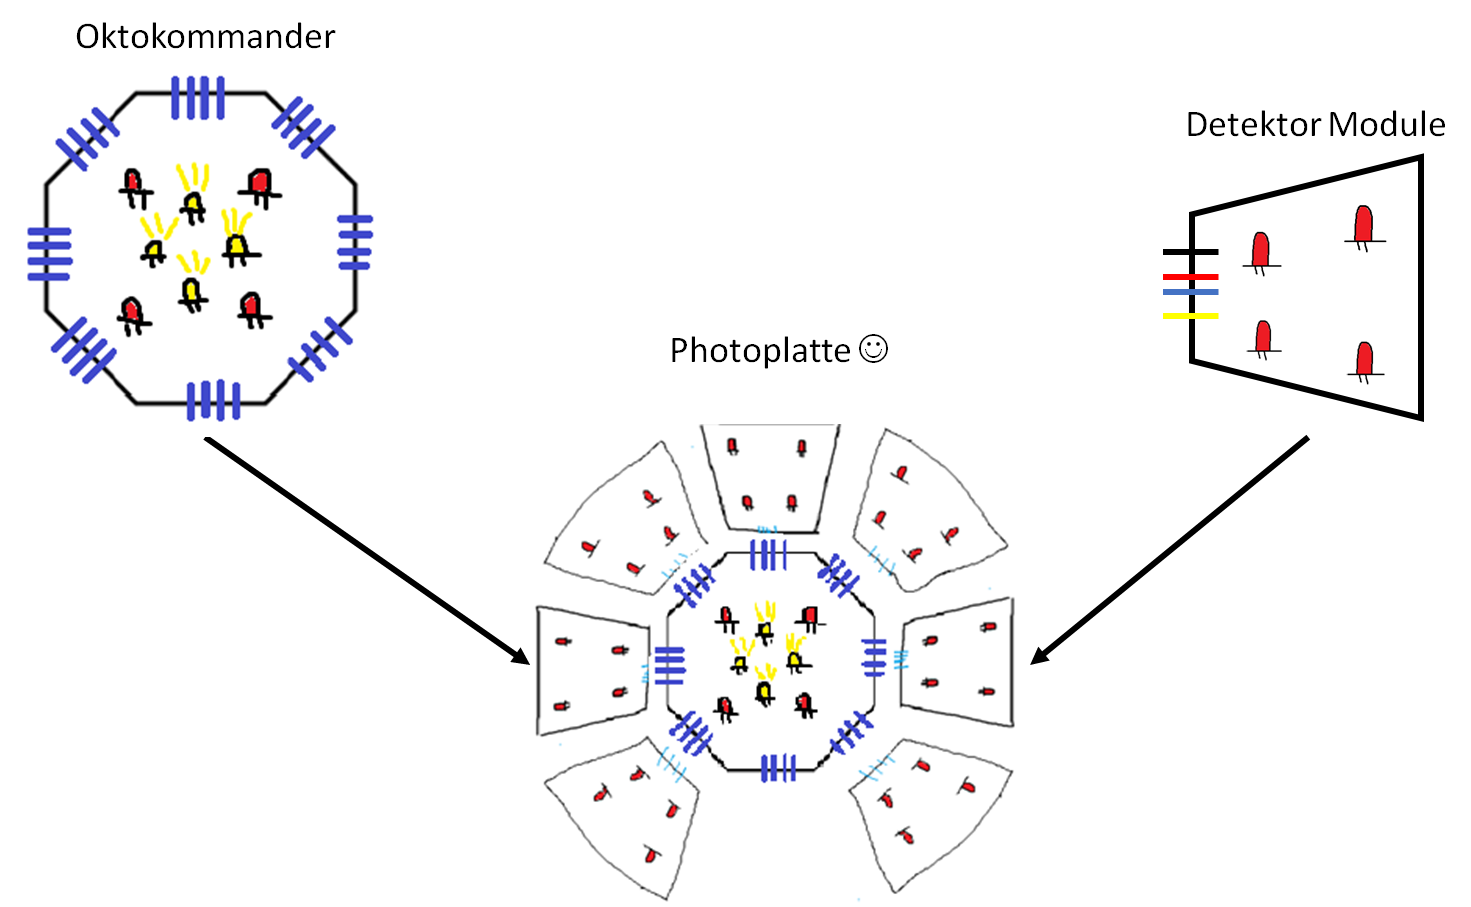
\includegraphics[scale=0.5]{figures/Photoplatte.png}

% -------------------------------------------------------------------------------------- %

\section{Oktokommander}
\label{sec:Oktokommander}

Der Oktokommander ist das Steuersystem der gesamten Photoplatte. In ihr befinden sich ein Arduino Micro, welcher die Signale aller Photodioden bearbeitet sowie einen i2c Expander. Durch den i2c Expander ist es möglich, jedes der Photodioden eine eigene Adresse zu zu weisen. Dies ist nötig, um die voneinander unabhängigen Signale der Photodioden richtig zuordnen zu können. Zusätzlich dazu befinden sich auf dem Oktokommander vier Infrarot LEDs sowie vier infrarot Photodioden. Um die vier infrarot Photodioden an zu steuern wird zusätzlich zum i2c Expander noch ein i2c Multiplexer sowie die dazu gehörende Verstärkerschaltung benötigt. 
\textcolor{red}{Erklärung der Komponenten im Bild}

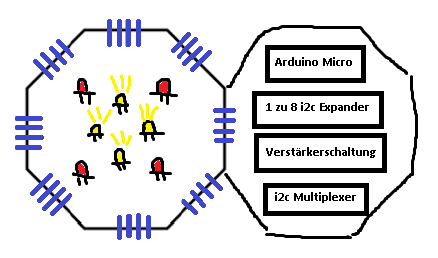
\includegraphics[scale=0.8]{figures/OktokommanderOffen.png}

Um den Oktokommander mit den Detektormodulen erweitern zu können wurden USB-2A Schnittstellen verwendet. Durch diese Schnittstellen können bis zu 7 Detektormodule, jeweils eines pro Seite  eingekoppelt werden. Um eine größere Platte zu konstruieren können noch weitere Detektormodule an den bereits vorhandenen Detektormodule angeschlossen werden.
\textcolor{red}{Erklärung der Komponenten im Bild}

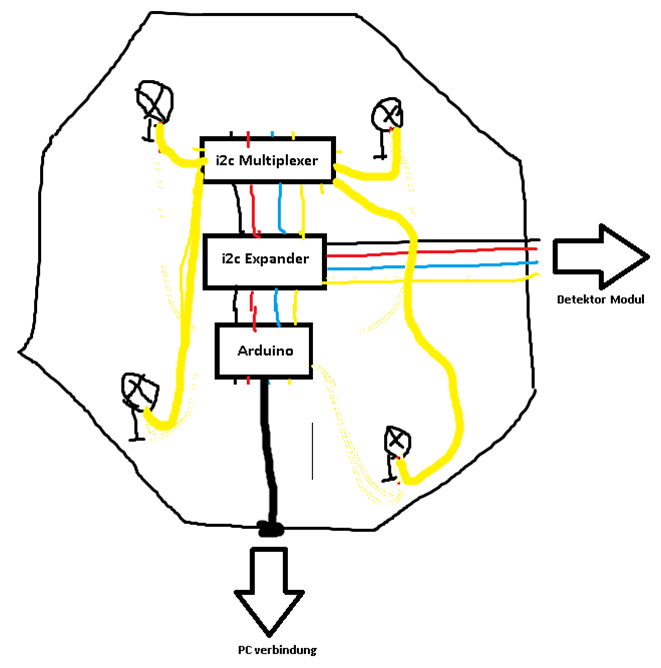
\includegraphics[scale=0.8]{figures/PrinzipskizzeOktokommander.png} 

% -------------------------------------------------------------------------------------- %

\section{Detektormodul}
\label{sec:Detektormodul}

Das Detektormodul besteht lediglich aus vier Photodioden und einem USB-2A Eingang. Dadurch kann das Detektormodul an den Oktokommander angeschlossen werden. Zur Ansteuerung der Photodioden wurde auch hier ein i2c Expander verwendet. 
\textcolor{red}{Erklärung der Komponenten der Bilder}

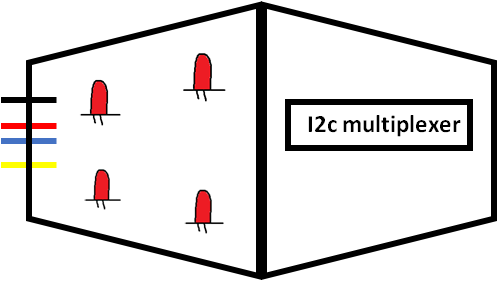
\includegraphics[scale=0.7]{figures/DetektormodulOffen.png}
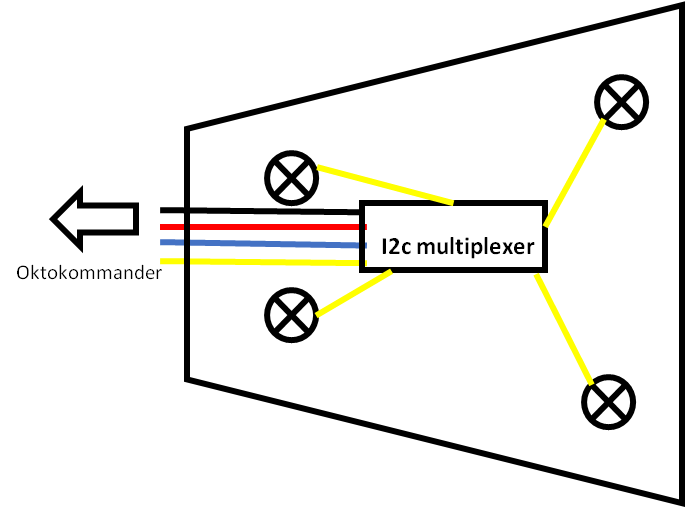
\includegraphics[scale=0.5]{figures/PrinzipskizzeDetektormodul.png}

% -------------------------------------------------------------------------------------- %

\section{Software}
\label{sec:Software}

